% Chapter 2

\chapter{Estado del Arte}
\label{capitulo2}

Sin la ciencia, no podría existir la ingeniería. Sin investigación y curiosidad acerca del entorno, no podría existir innovación y creatividad frente los problemas que se da. Es por tal motivo que el siguiente capítulo trata de un estudio del entorno en cuanto tecnologías en adición a trabajos e investigaciones previos que han sido realizados por terceros para en base a ello dar contexto a la investigación actual y aprender de lo bueno y malo de cada ascendente.

En la sección 2.1 de este capítulo, se presenta el marco teórico donde se realiza una investigación y estudia previa a las tecnologías y otros aspectos de entorno previo al planteamiento de una solución al problema introducido previamente. En la sección 2.2, se sigue con un estudio de trabajos relacionados a las temas abarcados en este trabajo de titulación mientras que en la sección 2.3 se realiza un estudio de sistemas similares en funcionalidad. Y finalmente se cierre el capítulo con la sección 2.4 donde se de una discusion y conclusion a todo lo analizado y presentado del capítulo con comparaciones de los mismos. 

% enumerar las secciones dentro mismo parafo 

\section{Marco Teorico}
Para llevar a cabo de forma exitosa el trabajo de titulación y entender el contexto del ambiente en que sea implementado es importante establecer una línea base de conocimiento que se ve a continuación y dividido de la siguiente forma:
\begin{description}
	\item[Aspectos de Propiedad Intelectual] que se topa con las licencias y culturas de código abierto y libre que se encuentra actualmente en el entorno.
    \item[Aspectos Ambientales del Entorno de Desarrollo] se trata de dar mejor contexto al entorno en el cual se encuentra la aplicación planteada. Esto incluye pero no está limitado a conceptos teóricos, aplicaciones y protocolos.
\end{description}

\subsection{Aspectos de Propiedad Intelectual}
Hoy en día, en un mundo cada vez más conectado y con cada vez más informacion compartida entre personas distintas, es importante conocer bien temas de derechos de autor y propiedad intelectual, no sólo para desarrollar y despues dar licencia a un trabajo de titulación, si no también para entender lo que se puede y no se puede hacer dentro de un entorno de desarrollo que cada vez involucra más algún codigo o trabajo que fue desarrollado alguna licencia abierta o libre.

\subsubsection{Software Libre}
Software Libre es un movimiento sociopolítico que busca liberar códigos fuentes. Se divide en dos campos que son: los de Open Source (Fuentes Libres) que quieren liberar código fuente sólo en base a los méritos de desarrollo colaborativo y los de Free/Libre Software (Software Libre) que buscan liberar código fuente en base a ciertos derechos de compartir, colaborar y tener control de lo que hacen sus dispositivos que se les pertenecen (su propiedad) para todos los usuarios que ocupan el software \citep{GNU-FLOSS-vs-FOSS} \citep{GNU-Open-vs-Free}. En el contexto de esta tesis, Software Libre se refiere al segundo campo, no al primero. Para el mismo, la fundación GNU con su fundador Richard M. Stallman define 4 libertades mínimas que deben ser cumplidas para constituir Software Libre y los cuales se los enumera desde el 0 hasta el 3 \citep{GNU-Freedom} \citep{GNU-Free-Software}:

\begin{enumerate}
  \setcounter{enumi}{-1}
  \item La libertad de ejecutar el programa para cualquier propósito que desee
  \item La libertad de estudiar cómo funciona el programa y poderlo modificar como desee. Un requisito para esta libertad es que el usuario tenga acceso al código fuente original.
  \item La libertad de distribuir copias del programa original con terceros.
  \item La libertad de distribuir copias de sus versiones modificadas a terceros. Un requisito para esta libertad es que el usuario tenga acceso al código fuente original.
\end{enumerate}

%\citep{GNU-Freedom} \citep{GNU-Free-Software}

Donde el software no cumpla con uno de los anteriores, ya deja de ser considerado libre. Sólo por ser software libre no significa que no puede ser comercializado, únicamente se requiere nuevos modelos de negocio los cuales si se los puede encontrar en uso diario \citep{GNU-Free-Software}. Como sociedad, Stallman argumenta, es importante proteger esas libertades porque avanzan la humanidad, como la libertad de expresión, ya que las libertades que se proponen proteger, buscan sostener una sociedad que trabaja por el bien de todos, no de solo unos pocos que saben más de la funcionalidad de ciertos aspectos tecnológicos \citep{GNU-Open-vs-Free}. En la época actual de gobiernos y empresas que espían sin vergüenza, se ha revivido el movimiento político y se ha convertido en algo más necesario debido a que todos tenemos y  queremos nuestro derecho a la privacidad \citep{GNU-Freedom}.


\paragraph{OAS}
OAS o Adopción de Software Libre es la tendencia que hay en el mundo empresarial de adoptar soluciones de tecnologías abiertas como los que ofrecen el mundo de software libre ya que las mismas pueden llegar a ser superiores en cuanto su eficacia y costo, que lo que ofrece su competencia comercial. Se estima que más del 78\% de instituciones usan software  de Fuentes Abiertas y menos del 3\% indican que no utilizan nada de software de fuentes abiertas. Eso demuestra un enorme mercado creciente y emergente a nivel mundial \citep{ACCEL-OAS}.

\paragraph{GNU}
El proyecto GNU fue lanzada por el señor Richard Mathew Stallman en el año 1983 con un fin de desarrollar en comunidad un sistema operativo que podría reemplazar los sistemas operativos UNIX de aquella época con algo que sería un 100\% software libre \citep{GNU-GNU-OS}. Pero nunca terminaron todo el proyecto, específicamente el núcleo del sistema operativo, conocido como GNU Hurd, porque antes llegó otro núcleo desarrollado por un joven estudiante de sistemas llamado Linus Torvalds quien llamó su clon libre de UNIX, Linux, y de esta forma, unida con todo lo que se había desarrollado el proyecto GNU, se formó un sistema operativo completamente libre \citep{GNU-GNU-Linux}.

\paragraph{GPL}
Aunque es la licencia más común en proyectos de software libre y usada para una mayoría de ellos, especialmente dentro del proyecto GNU, la GPL o GNU Public License no es la única licencia libre que existe \citep{GNU-Licenses}. Fue diseñada específicamente en la década de los 1980s para proteger la libertad de los usuarios de software \citep{GNU-Open-vs-Free}. La última versión, GPLv3 fue publicada en Junio de 2007 y construye encima de versiones anteriores para tratar de asegurar de mejor manera las 4 libertades que tiene que garantizar cualquier licencia que quiere ser software libre \citep{GNU-GPL-Guide} \citep{GNU-GPL}.

\subsection{Aspectos Ambientales del Entorno de Desarrollo}
El contexto dentro del cual se desarrolla cualquier proyecto y sobre todo conocer las tecnologías existentes dentro de un ambiente en los proyectos tecnológicos, son puntos importantes que se debe tomar en cuenta previo a la ejecución del mismo. Es por tal motivo que a continuación se presenta algunas de las tecnologías con que se va a encontrar el proyecto y la teoría detrás de ellos.

\subsubsection{Tipos de Recurso de Aprendizaje}
\begin{table}[h!]
	\small
    \begin{tabular}{|p{0.08\textwidth}|p{0.92\textwidth}|}
        \hline
        Concepto & Definición \\
        \hline
        LA & LA es un activo de aprendizaje el cual representa un archivo que no llega al nivel de un objeto de aprendizaje. También se los guarda en repositorios de objetos de aprendizaje \citep{GOVIEW-LOR}. \\
        \hline
        LO & LO es un objeto de aprendizaje y es un recurso que ayuda a los estudiantes con su aprendizaje, por ejemplo un tema (que se puede enseñar con diapositivas, enlaces, documentos, etc), pruebas, exámenes, etc \citep{GOVIEW-LOR}. \\
        \hline
        LOR & LOR es un repositorio de objetos de aprendizaje unidos por docentes y otros profesionales educativos para enseñar a sus alumnos de la mejor forma posible \citep{GOVIEW-LOR}. \\
        \hline
    \end{tabular}
	\caption{Tipos de Recurso de Aprendizaje.}
    \label{tipos-recurso-aprendizaje}
\end{table}

\subsubsection{MOOC}
MOOCs o Cursos Online Masivos Abiertos son cursos abiertos en línea que guían estudiantes paso a paso en su aprendizaje sin límites como costos, fronteras o culturas. Los mismos usan expertos del área en cuestión para dar el mejor calidad de educación possible a través de videos, pruebas, foros, redes sociales, charlas y artículos que promuevan debate y reflexión \citep{UEA-What-is-a-MOOC}.

\subsubsection{CMS}
Un sistema de gestión de cursos es una colección de herramientas que ayudan proveer un ambiente en línea para interacciones entre integrantes de una clase. Esto puede incluir espacio para publicar anuncios, recolección de deberes, gestión de notas tanto para que docentes puede calificar sus alumnos y los mismos alumnos pueden ver sus notas en tiempo real, integración con sistemas de correos institucionales, chat en vivo y foros que permiten responder a entradas previas  \citep{Vanderbilt-Course-Management-Systems}.

\subsubsection{LMS}
Según Mindflash, un vendedor de sistemas educativos \citep{MINDFLASH-ABOUT}, los LMS, o Sistemas de Gestión de Aprendizaje, son herramientas muy útiles para instituciones educativas y otras entidades económicas que lo apoyen para organizar y gestionar recursos educativos, estudiantes, docentes y cursos. Las mismas son un aspecto crítico de la tendencia que tiene el sector educativo a digitalizarse que se puede ver en la aproximadamente 600 LMS que existen para elegir. Características comunes entre ellos incluyen: \citep{MINDFLASH-LMS}
\begin{itemize}
	\item Listas de Estudiantes para tomar asistencia entre otras interacciones que puede haber entre estudiantes y sus profesores.
    \item Matrículas
    \item Gestión de Documentos
    \item Soporte para Educación Distribuido; por ejemplo alumnos y/o docentes a distancia
    \item Calendarios de Curso para dar a conocer cronogramas, fechas para pruebas, exámenes y deberes.
    \item Interacción Estudiantil a través de correo electrónico, foros y chat.
    \item Comprobación de Conocimiento de Alumnos con pruebas y exámenes.
    \item Sistemas de Calificación que pueden ser automatizados (en casos objetivos), manuales por parte del docente (para casos más subjetivos) y híbridos cuando un profesor ofrece ambos casos en un curso.
\end{itemize}
%\citep{MINDFLASH-LMS}

\paragraph{Moodle}
Moodle es un LMS de software libre, licenciada bajo el GPLv3 \citep{MOODLE-GIT-License},  que ofrece los caracteristicas típicas de un LMS como herramientas de colaboración (Wikis, Foros, Glosarios, etc), gestión de y interacción con estudiantes (notificaciones, gestión de progreso y notas, etc), en adición a gestión de usuarios y matrículas \citep{MOODLE-DOCS-Features}. Actualmente es lo que usa la UTPL con sus Docentes y Alumnos a través del Entorno Virtual de Aprendizaje \citep{Lopez-Jorge}.

\paragraph{OpenCampus}
OpenCampus es un sistema para instituciones educativas para ayudar a gestionar sus estudiantes y procesos a través de una combinación de OAS y software propietario con un fin de proveer mejor acceso a recursos educativos a todos \citep{OpenCampus-Tecnology}, el mismo integra sistema de gestión de campus (CMS), gestión de escuelas de postgrado (GSM), sistema de gestión de aprendizaje (LMS), gestión de escuelas de medicina, sistema de aprendizaje electrónica, gestión de salud en el lugar de trabajo, gestión de objetivos, sistema de gestión de información estudiantil, gestión de clases, sistema de gestión de dato de investigación, sistema de gestión de ensayos clínicos, gestión de becas de investigación y gestión de laboratorios \citep{OpenCampus-Home}. De esta manera ofrece características comunes de los LMS como exámenes, cursos en línea, rastreo académico para docentes, alumnos y administradores \citep{OpenCampus-Tecnology} \citep{OpenCampus-Universities}. La UTPL está ocupando esta tecnología actualmente para ofrecer “cursos en línea… de forma abierta y libre” \citep{UTPL-OpenCampus}.

\subparagraph{Open edX}
Una organización sin fines de lucro famosa por sus cursos abiertos masivos (MOOCs), EdX, se ha liberado con una licencia libre su plataforma bajo el nombre Open edX. El mismo ofrece:
\begin{itemize}
	\item CMS para gestionar varios cursos
    \item LMS para presentar contenido a estudiantes y profesores
    \item Open edX Studio para el diseño de cursos desde su contenido y políticas de calificación hasta el horario que seguirá y el equipo de docentes.
    \item Un plataforma para MOOCs
    \item XBlock para construir arquitecturas de componentes donde docentes mismos pueden agregar funcionalidad a su curso sin meterse mucho al resto del sistema.
    \item Foros
    \item Recolección de Datos para la toma de decisiones estratégicas
\end{itemize}
Según la documentación del mismo, Open edX utiliza una arquitectura de NGinx con Gunicorn y Django. Para el despliegue del mismo en entornos de desarrollo se ofrece una máquina virtual preconfigurada denominado “DevStack” \citep{edX-About-Open-edX}. Como tecnología de backend, el OpenCampus de la UTPL utiliza Open edX \citep{Lopez-Jorge}.

\subsubsection{LTI}
LTI es un estándar para asegurar interoperabilidad entre sistemas educativos. Fue diseñada y es gestionado por IMS Global Learning Consortium \citep{IMS-Global-LTI}, un conjunto de instituciones y organizaciones que desean mejorar procesos educativos \citep{IMS-Global-Members}, con el fin de simplificar el proceso de interconección de aplicaciones de aprendizaje (conocidos en el estándar como Herramientas [de aprendizaje]), como los que saben ofrecer terceros, con ambientes educativos (conocidos en el estándar como Consumidores de Herramientas [de aprendizaje]) que pueden ser sistemas de gestión de aprendizaje (LMS), portales de aprendizaje, repositorios de objetos de aprendizaje (LOR), o otros ambientes educativos \citep{IMS-Global-LTI}. Moodle ofrece una implementación estándar para comunicarse con sistemas de terceros \citep{MOODLE-DOCS-Features}.

\subsubsection{Sistema de Control de Versionamiento}
Un sistema de control de versiones mantiene y organiza un historial de versiones de uno o más archivos con el fin de poder intercambiar entre versiones rápidamente. Son muy usados para quienes trabajan con código fuente y también artistas \citep{PROGIT-Git-VCS} que necesitan llevar un historial de sus obras de arte, pero su utilidad no termina allí ya que son diversos los grupos que pueden aprovechar los beneficios que ofrecen estos sistemas. El sistema màs común que sabe usar los seres humanos actualmente es copiar archivos que deseen versionar, típicamente dándoles una nueva ubicación o nombre dado que es una solución muy simple para lograr versionar, pero eso puede ser peligroso ya que es muy fácil trabajar sobre una versión incorrecta, por lo que se inventaron los sistemas de control de versionamiento, programas especializados en ayudar los seres humanos llevar una historial de versiones en uno o más archivos.

Inicialmente esos eran sumamente locales, como RCS, que mantiene una base de datos con todas las versiones (almacenadas como los cambios que hubieron en comparación con la versión anterior, una práctica conocida como respaldo incremental) y en base a eso permitir acceso a la versión actual o cualquiera de los otros guardadas previamente, mira figura \ref{LVCS}. \citep{PROGIT-Git-VCS}.

\begin{figure}
  \begin{center}
    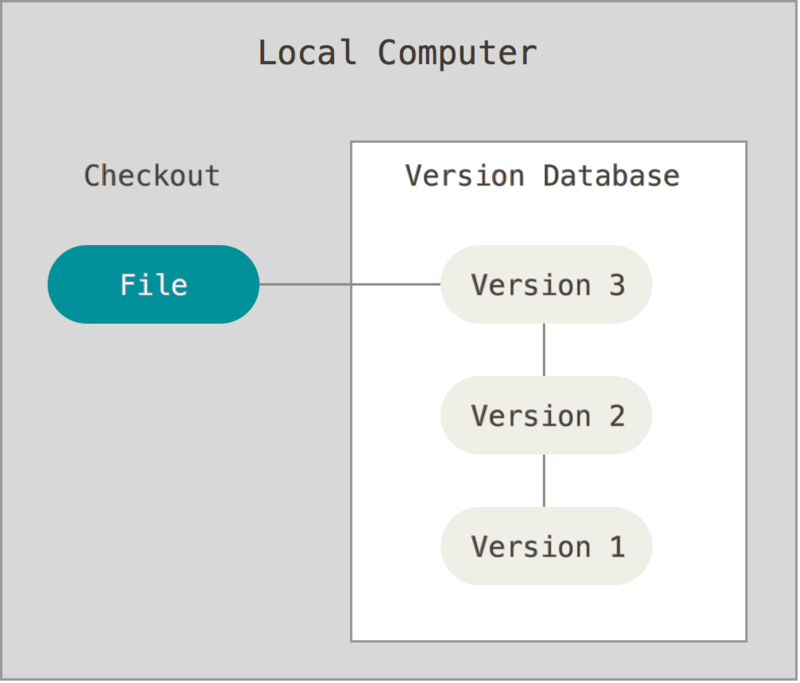
\includegraphics[width=0.5\textwidth]{Figures/lvcs.png}
  \end{center}
  \caption{Sistema de Control de Versionamiento Local. \citep{PROGIT-Git-VCS}.}
  \label{LVCS}
\end{figure}

Después se dieron cuenta que seria bueno poder colaborar sobre las mismas versiones entonces se inventó lo que se conoce como Sistemas de Control de Versionamiento Centralizados los cuales permiten un alto grado de control y seguridad sobre quién puede editar y cuando puede editar que dentro de la base de datos de contenido ya que las mismas siguen un modelo arquitectónico cliente-servidor \citep{PROGIT-Git-VCS}. Eso ha resultado que en empresas grandes que necesitan desarrollar sistemas grandes en paralelo con un cierto grado de seguridad, les resulta bien usar un sistema de control de versionamiento de esta clase aunque esto está cambiando ya que las empresas están dándose cuenta que pueden optar por una solución híbrida \citep{CollabNet-Dist-or-Cent}. Ejemplos de estos CVCS son CVS, Subversión y Perforce. Pero el problema viene a ser que todo el repositorio tiene un solo punto de falla porque si cae el servidor o le pasa algo, se pone en riesgo la productividad continua de quien colabora y en el peor de los casos, la integridad del repositorio. Esta propiedad se puede ver en la figura \ref{CVCS} \citep{PROGIT-Git-VCS}.

\begin{figure}
  \begin{center}
  	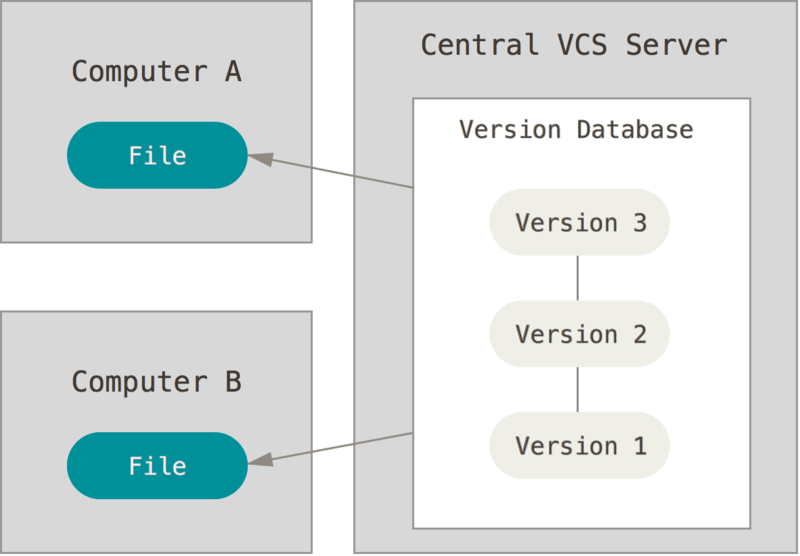
\includegraphics[width=0.5\textwidth]{Figures/cvcs.png}
  \end{center}
  \caption{Sistema de Control de Versionamiento Centralizado. \citep{PROGIT-Git-VCS}.}
  \label{CVCS}
\end{figure}

Con la explosión de desarrollo de software libre, hubo una necesidad de poder trabajar grandes cantidades de personas desconocidas en paralelo \citep{raymond1999cathedral}, y para resolver este problema y también la de integridad de datos que presenta el único punto de falla de los Sistemas de Control de Versionamiento Centralizado, se inventó Sistemas de Control de Versionamiento Distribuidos como Git, Mercurial, Bazaar y Darcs. Cada repositorio es un espejo de los demás en una arquitectura distribuida o red de iguales. Con esta arquitectura (mira figura \ref{DVCS}), ningún nodo viene a ser un punto de falla ya que se puede espejar entre cualquiera de ellos debido al hecho de que todos tienen una copia local de todo lo que tienen los demás \citep{PROGIT-Git-VCS}. 

\begin{figure}
  \begin{center}
      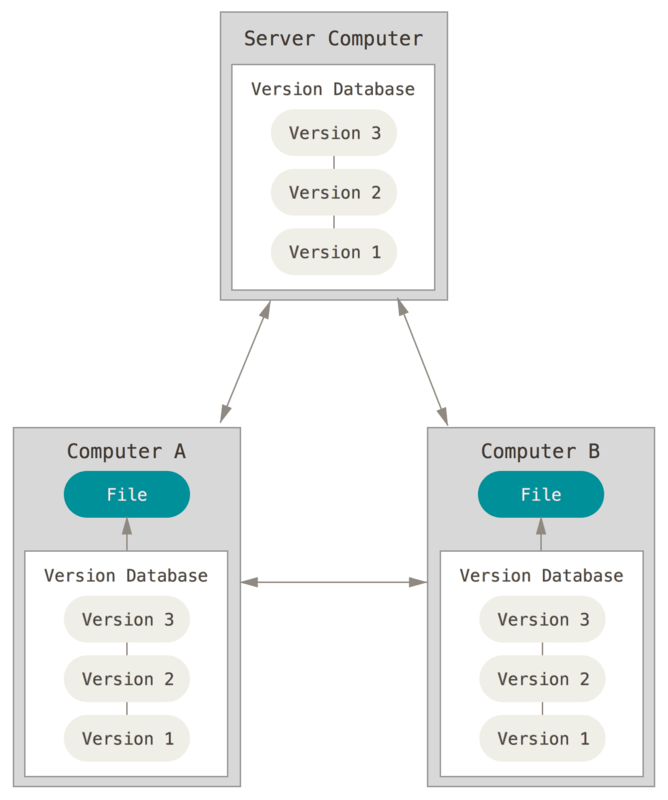
\includegraphics[width=0.5\textwidth]{Figures/dvcs.png}
  \end{center}
  \caption{Sistema de Control de Versionamiento Distribuido. \citep{PROGIT-Git-VCS}.}
  \label{DVCS}
\end{figure}

\subsubsection{Git}
Git es un sistema de control de versiones distribuido que a diferencia de otros VCS guarda con cada versión una copia entera de los archivos modificados (otros sistemas de control de versionamiento saben guardar solo las diferencias entre versiones de forma incremental, mira la diferencia entre la figura \ref{VCS-Incremental} y la figura \ref{VCS-Backup}) \citep{PROGIT-Git-Intro}.

\begin{figure}
  \begin{center}
      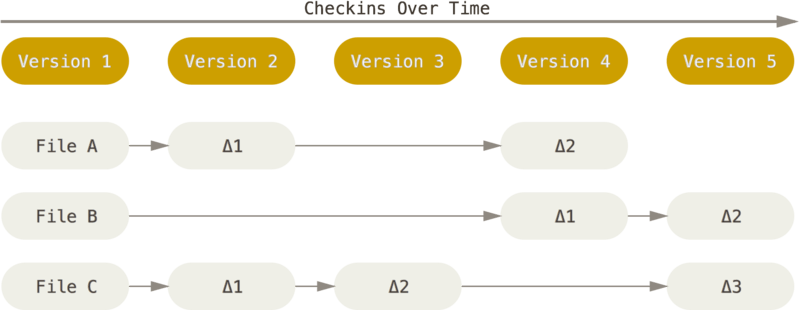
\includegraphics[width=\textwidth]{Figures/vcs-incremental.png}
  \end{center}
  \caption{Sistema de Control de Versiones llevado de forma incremental. \citep{PROGIT-Git-Intro}.}
  \label{VCS-Incremental}
\end{figure}

\begin{figure}
  \begin{center}
      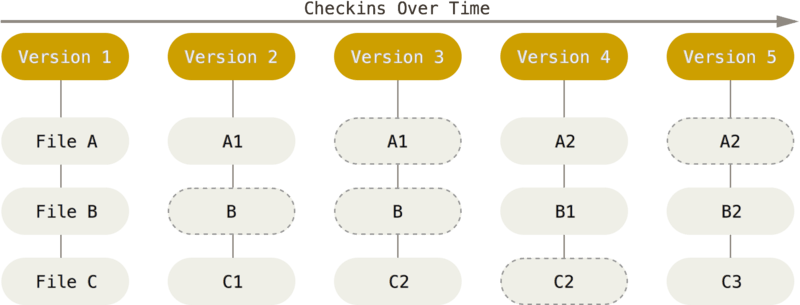
\includegraphics[width=\textwidth]{Figures/vcs-backup.png}
  \end{center}
  \caption{Sistema de Control de Versiones llevado con archivos enteros. \citep{PROGIT-Git-Intro}.}
  \label{VCS-Backup}
\end{figure}

Esto hace que Git se convierte más en como un pseudo sistema de ficheros que un simple VCS. Además significa mayor integridad de los datos guardados a costo de mayor consumo de almacenamiento. Trabaja de esta manera distribuida, es decir el repositorio existe en esta forma en todo lado donde se encuentra y por lo tanto la mayoría de operaciones de Git se puede realizar de manera local sin ninguna conexión de red \citep{PROGIT-Git-Intro}.
Volviendo al tema de integridad de datos, Git utiliza SHA-1 como algoritmo criptográfico para calcular los hash de cada cambio que se realiza en base a una combinación de qué información contiene el cambio, su metadata como autor, fecha, hora y fecha en adición a los SHA-1 de su(s) cambio(s) padre(s)\footnote{La mayoría de commits solo tienen un padre, pero aquellos que unen varios historiales, tienen dos padres} de tal forma que es difícil si no prácticamente imposible\footnote{Un equipo de investigación de Google y CWI Amsterdam ha encontrado una vulnerabilidad que recién publicaron y les permite atacar SHA-1 y encontrar colisiones hash \citep{Shattered-Paper}} para un atacante modificar el historial sin dejar evidencia de lo que se ha hecho. Por defecto funciona así \citep{PROGIT-Git-Intro}, pero si uno desea asegurar la integridad del historial aún más, se integra Git con GPG para ofrecer mayor seguridad ya que con eso se puede firmar digitalmente cambios realizados para demostrar su autenticidad \citep{PROGIT-Git-GPG}.

La mayoría de operaciones normales  que se hacen en Git no eliminan datos ya guardados en el repositorio previamente lo cual lo hace una buena herramienta para personas que recien esta entrando al mundo de Sistemas de Control de Versionamiento y permite que se pueda recuperar de la mayoría de errores que se puede cometer y una recuperación casi garantizado de datos “perdidos”. Eso es gracias en parte a la filosofía que se refleja en el diseño del mismo ya que una prioridad primordial era la integridad de los datos \citep{PROGIT-Git-Intro}.

Cada repositorio de Git trabaja con tres fases que son el directorio de trabajo donde se realiza cambios, una área de preparación donde se marca cambios listos para guardar y una base de datos junto un sistema de ficheros donde se guardan los cambios. Al saltarse entre versiones, se sobreescribe los contenidos del directorio de trabajo con lo que se extrae del sistema de ficheros que tiene los cambios guardados. Esas tres fases y su relación se puede ver en la figura \ref{Git-Fases} \citep{PROGIT-Git-Intro}.

\begin{figure}
  \begin{center}
      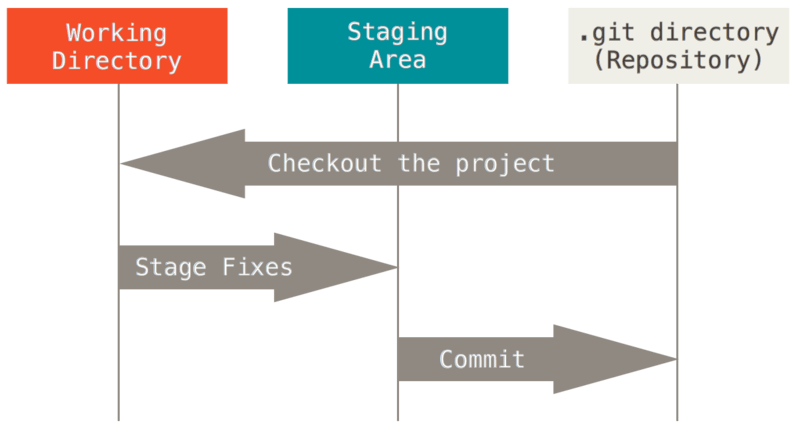
\includegraphics[width=0.5\textwidth]{Figures/git-fases.png}
  \end{center}
  \caption{Los tres fases de Git y sus relaciones. \citep{PROGIT-Git-Intro}}
  \label{Git-Fases}
\end{figure}

\paragraph{GitLab}
GitLab es un servidor de Git ofrecido por GitLab Inc. Se ofrece en dos versiones: una versión gratis \citep{GitLab-Products} de código abierto liberado bajo el nombre GitLab Community Edition (GitLab CE) y una versión pagada que forma la línea principal de negocio de GitLab Inc. que lo venden bajo el nombre GitLab Enterprise Edition (GitLab EE) \citep{GitLab-About}. También proporcionan hosting de las mismas versiones alojados por ellos en GitLab.com (alli se puede usar GitLab EE gratis \citep{GitLab-GitLab.com} \citep{GitLab-Products}) y en GitHost.io (donde se puede arrendar servidores para alojar instancias de GitLab CE o EE y su respectivo infraestructura de apoyo \citep{GitHost.io}) \citep{GitLab-About}. Actualmente la Universidad Técnica Particular de Loja utiliza un servidor de GitLab CE como su instancia institucional de Git \citep{UTPL-GitLab}.

\subsubsection{Virtualización}
Virtualización es la creación de recursos virtuales en software para usar los mismos en lugar de un recurso físico. Este puede ser usado en áreas diversas como aplicaciones, servidores, almacenamiento y redes. Según la empresa VMware, que se dedica a vender productos de virtualización, la misma es la estrategia más efectiva para reducir costos de TI mientras que se aumenta la eficiencia y agilidad de un negocio de cualquier tamaño. Llegan a esta conclusión porque es tan común que se ha convertido en estándar industrial que solo se ocupa en entre 5\% y 15\% de la capacidad de los servidores debido a que se les pone solo un sistema operativo y aplicación a la vez. Virtualización permite resolver estas deficiencias en permitir la división lógica de equipos y distribuir estas partes donde más se los necesitan para aumentar la tasa de eficiencia y reducir la cantidad de recursos físicos necesarios. Con esta clase de tecnología, se puede reducir y en algunos casos eliminar tiempo fuera de servicio. Las facilidades de portabilidad y agilidad de ajustar recursos hace que se puede reducir los tiempos y costos de administración. Se domina hipervisor un software que gestiona virtualización \citep{VMWare-Virtualization}. Tholeti y IBM tienen un concepto similar de reducción de recursos físicos y gastos de operación, como se indica en la figura \ref{IBM-Virtualization}, la optimización de recursos físicos después de la virtualización.

\begin{figure}
  \begin{center}
      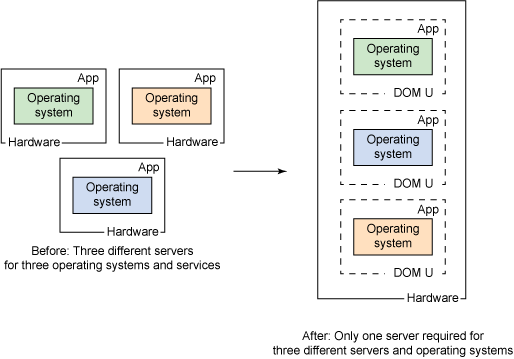
\includegraphics[width=0.5\textwidth]{Figures/ibm-virtualization.png}
  \end{center}
  \caption{Antes y después de virtualizar aplicaciones. \citep{IBM-Hypervisors}.}
  \label{IBM-Virtualization}
\end{figure}

\paragraph{Las Máquinas Virtuales}
Una Máquina Virtual es una sistema computacional entera con sistema operativo y aplicación corriendo sobre recursos virtuales. Por lo tanto cada máquina virtual es completamente aislada e independiente de los demás de tal forma que se puede tener varios sistemas operativos y aplicaciones corriendo sobre un solo servidor físico. Eso permite tener varias características importantes:
\begin{description}
	\item[División de Recursos] Se puede dividir recursos físicos entre varios sistemas operativos corriendo sobre la misma máquina.
    \item[Aislamiento] Proveer mayor seguridad en prevenir o restringir acceso entre las varias máquinas virtuales.
    \item[Encapsulación de Persistencia] Todo el estado de la máquina virtual se lo puede guardar en archivos, los mismos que pueden ser sincronizados entre varios equipos o ubicaciones.
    \item[Independencia de Hardware] Se puede usar la máquina virtual en cualquier hipervisor que lo soporte.
\end{description}
Todo estas caracteristicas anteriores permiten la consolidación de servidores para utilizar menos servidores y cortar costos \citep{VMWare-Virtualization}.

\paragraph{Virtualización de Servidores}
Con virtualización de servidores, se puede reducir el número de servidores necesarios dentro de una granja, especialmente cuando los mismos son miembros de un cluster que realiza balanceo de recursos frente su carga para optimizar la eficiencia de toda la granja \citep{VMWare-Virtualization}.

\paragraph{Virtualización de Redes}
Con virtualización de redes se puede simular todo el tráfico y funcionamiento de una red sin mayor retardo. Se puede virtualizar interfaces de red, los switch, routers, cortafuegos, balanceadores de carga, VPNs y más. Como los otros tipos de virtualización, esta ofrece los mismos beneficios de independencia, costos y escalabilidad \citep{VMWare-Virtualization}.

\paragraph{Virtualización de Escritorios}
Virtualización de Escritorios se trata de usar recursos centralizados para dar escritorios de trabajo a usuarios remotos. Esto permite a cualquier organización reducir sus gastos tecnológicos debido a que el mismo permite menor inversión en tecnología para la misma cantidad de usuarios mientras al mismo tiempo facilita temas de administración de los equipos de los empleados en una organización y seguridad de la información de la misma \citep{VMWare-Virtualization}.

\subsubsection{Hipervisores}
Un hipervisor es una capa intermedia de software que gestiona la interacción entre lo virtualizado y hardware o otro software que ayuda realizar las peticiones de lo virtualizado \citep{VMWare-Virtualization}. De la misma manera, el mismo hipervisor se encargan de seguridad para asegurar que lo que sea virtualizado no pueda salir de su ambiente y atacar otras partes virtualizados o no virtualizados \citep{VMWare-HypervisorSecurity} \citep{IBM-KVM-Security}. La figura \ref{IBM-HypervisorTypes} muestra los tipos clásicos de hipervisor que se presentan a continuación, los hipervisores de tipo 1 que son a bajo nivel en lugar de un sistema operativo y los hipervisores de tipo 2 que son una aplicación montado encima de un sistema operativo.

\begin{figure}
  \begin{center}
      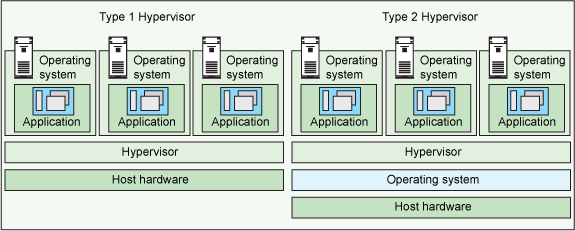
\includegraphics[width=\textwidth]{Figures/ibm-hypervisortypes.png}
  \end{center}
  \caption{Tipos Clásicos de Hipervisor \citep{IBM-Hypervisors}.}
  \label{IBM-HypervisorTypes}
\end{figure}

\paragraph{Hipervisores de Tipo 1}
Un Hipervisor de Tipo 1 se ejecuta directamente sobre hardware física \citep{IBM-Hypervisors} y por lo tanto puede llegar a conseguir mejor rendimiento y seguridad pero a un costo de requerir en muchos casos mayor configuración y administración para poder alcanzar su rendimiento óptimo.

\subparagraph{Xen}
Xen es un hipervisor de tipo 1, que corre directamente sobre hardware. Es el único hipervisor de su clase que es completamente disponible bajo una licencia abierta y forma una base por muchas aplicaciones comerciales y no comerciales como virtualización de servidores, IaaS, virtualización de escritorios, aplicaciones de seguridad, y dispositivos embebidos. Dentro del mercado, es la tecnología detrás de las nubes más grandes \citep{Xen-Project-Overview}. En la figura \ref{arq-xen} se puede encontrar la arquitectura Xen física/lógica para entender mejor como funciona la misma.
 
Para el mismo, se considera las siguientes características:
\begin{itemize}
	\item La implementación y uso de un micronúcleo que ocupa un mínimo de memoria y tiene interfaz externa limitado el cual ayuda proporcionar mayor seguridad y estabilidad en comparación con otros hipervisores. El hipervisor en si esta escrito en menos de 150 KLOCs que para un sistema operativo es muy liviano. Puede ser tan liviano porque no necesita tener conocimientos de operaciones de entrada/salida como redes o almacenamiento debido a que Dom0 se encargará de estos tareas. Al mismo tiempo, las demás máquinas virtuales no son privilegiados y siempre tienen que comunicarse con Dom0 para realizar cualquier operación con respecto al hardware físico. Por lo tanto la muerte del Dom0 es fatal para todas las máquinas que están en el Hipervisor.
    \item La arquitectura de Xen ocupa una maquina virtual que se domina Dom0 el cual contiene todos los drivers para el hardware y también la herramientas necesarias para ejercer control sobre todo el hipervisor. Estás funcionalidad son independientes del sistema operativo motivo por el cual que el sistema operativo residente del Dom0 puede ser Linux, una BSD, OpenSolaris, etc\ldots
    \item Como los drivers que controlan hardware física existen dentro de una máquina virtual, se los consideran drivers aislados. En caso de que pase algo, solo hay necesidad de reiniciar la máquina afectada, el resto del sistema puede seguir funcionando normalmente.
    \item Con una tecnología llamada paravirtualización, en lugar de optimizar al nivel de hipervisor se optimiza los sistemas operativos que son virtualizados para de esta manera mejorar su rendimiento incluso en hardware que no tiene soporte para virtualización. \citep{Xen-Project-Overview}.
\end{itemize}

\begin{figure}
  \begin{center}
      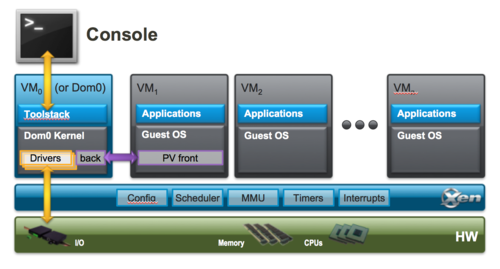
\includegraphics[width=\textwidth]{Figures/arq-xen.png}
  \end{center}
  \caption{La arquitectura de Xen. \citep{Xen-Project-Overview}.}
  \label{arq-xen}
\end{figure}

\paragraph{Hipervisores de Tipo 2}
Un Hipervisor de Tipo 2 se ejecuta por encima de un sistema operativo que le ayuda con su gestión interna como si fuera una aplicación más \citep{IBM-Hypervisors} lo que hace este tipos de hipervisores más lentos que hipervisores de tipo 1 (por tener un mayor número de capas y también por virtualizar partes del hardware) pero a su vez más fáciles de configurar y administrar. El mismo hecho de ejecutar por encima de un sistema operativo también vulnera la seguridad de todo el sistema en proveer un superficie de ataque más grande para actores maliciosos.

\subparagraph{Qemu-KVM}
QEMU es un proyecto de software abierto con el fin de crear un emulador y virtualizador de procesadores de varias arquitecturas para una variedad de sistemas operativos. Permite el uso de backends como KVM o Xen para dar rendimiento casi nativo \citep{QEMU}. Aunque su despliegue normal requiere un sistema operativo, basado en Linux, intermedio debido a que es un módulo que se integra directamente en el núcleo de la misma sistema operativo, Wilson et. al. consideran KVM como un hipervisor de tipo 1 debido a sus características y implementación a bajo nivel cerca al nivel hardware física, mientras que su arquitectura lo hace aparecer como un hipervisor de tipo 2, que es como se lo está considerando aquí dentro del contexto de este trabajo (mientras que otros autores lo consideran un hipervisor de tipo 1.5, ni uno ni el otro si no algo híbrido dentro de la taxonomía de hipervisores). KVM es la “hipervisor estratégica para IBM” debido a (1) su bajo costo por ser tecnología completamente abierta, (2) su alta evolución y madurez, (3) alta evolución y madurez de Linux (su tecnología fundamental atras), (4) eficiencia y rendimiento alto, (5) una comunidad de desarrollo muy activa y responsable frente fallos de seguridad, (6) la idea de que muchos ojos viendo código lo hace más seguro\footnote{Uno de las características principales de Código Abierto}, (7) varias tecnologías de seguridad que integra que falta la competencia, (8) mayor flexibilidad que ofrece frente otros hipervisores competidores y (7) control que IBM puede ejercer sobre el proyecto de KVM \citep{IBM-KVM-Security}. En la figura \ref{KVM-Arq}, se puede encontrar la arquitectura lógica para entender visualmente la funcionalidad de la misma.

\begin{figure}
  \begin{center}
      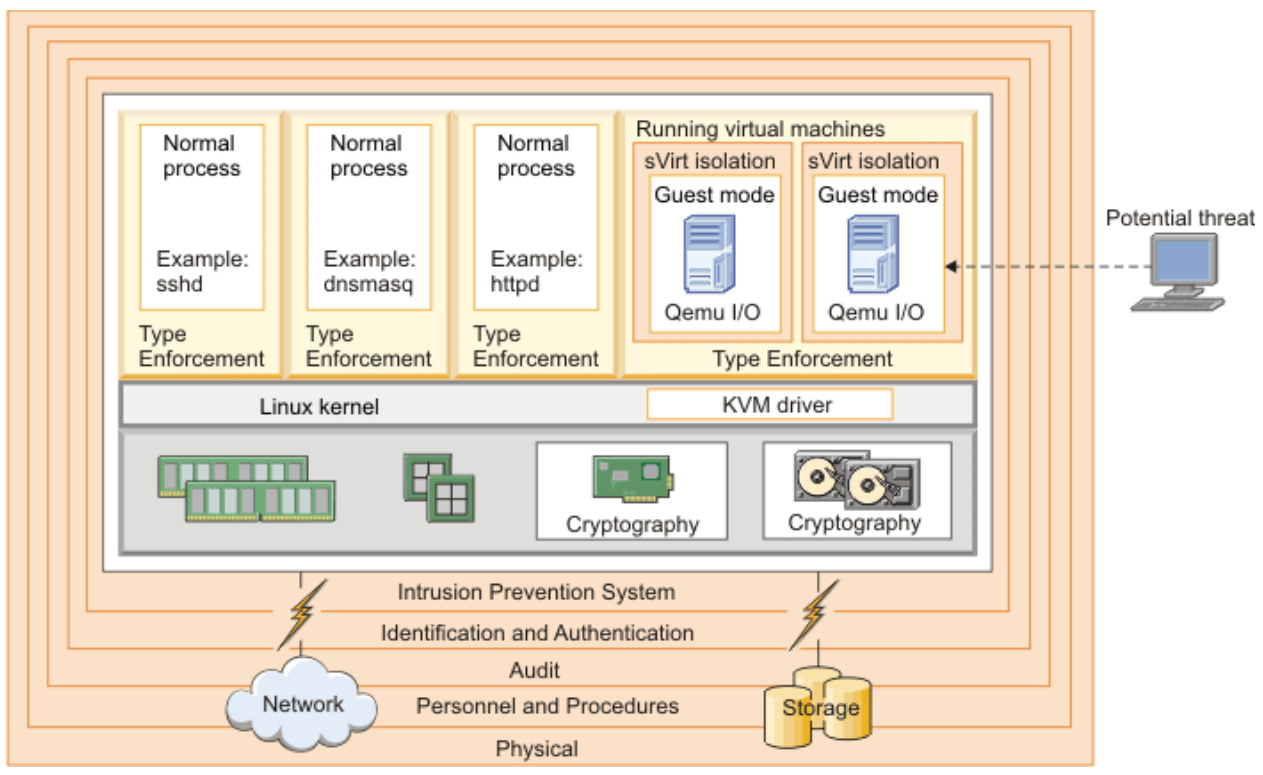
\includegraphics[width=\textwidth]{Figures/kvm-arq.png}
  \end{center}
  \caption{Arquitectura de KVM/QEMU. \citep{IBM-KVM-Security}.}
  \label{KVM-Arq}
\end{figure}

\subparagraph{VirtualBox}
VirtualBox es un hipervisor para virtualización de arquitecturas estándar x86 y x86\_64 tanto para uso casero como uso empresarial. Para ello ofrece muchas características, rendimiento optimizado, y un gran número de sistemas operativos que soporta tanto para virtualizar como para ser virtualizados todo bajo una licencia de software libre, la GPL versión 2 \citep{VirtualBox}. Su arquitectura de ser montado encima de cualquier sistema operativo y apoyarse en ello para realizar operaciones por parte de un sistema operativo y hardware virtualizado hacen este hipervisor un ejemplo clásico de un hipervisor de tipo 2.

\paragraph{Virtualización a Nivel de Sistema Operativo (Contenerización)}
Desde la antes de la incepción de los sistemas Linux, los sistemas de la familia Unix han tenido un mecanismo de aislamiento conocido como chroot el cual genera un espacio aislado de usuario para contener alguna aplicacion o varias aplicaciones mientras que todos siguen compartiendo el mismo sistema operativo o kernel por detrás. La tendencia de contenerización que existe hoy en día sigue por la misma línea pero lo implementa de una forma aún más avanzada. Eso permite a muchos usuarios que se desconfían mutuamente unos en otros utilizar el mismo hardware mientras que al mismo tiempo quedan completamente aislados unos de otros con menor impacto al rendimiento o una necesidad de hardware que soporta la carga adicional que virtualizacion genera \citep{Teimouri-Davoud-OS-level-virt}, mira la figura \ref{que-son-contenedores}. Algunos sistemas de este tipo de aislamiento que son populares hoy en día son:
\begin{multicols}{3}
  \begin{itemize}
      \item chroot
      \item Docker
      \item LXC
      \item LXD
      \item Linux-VServer
      \item OpenVZ
      \item Solaris Containers
      \item FreeBSD jail
      \item Hyper-V containers (Microsoft)
      \item Photon (VMware)
  \end{itemize}
\end{multicols}
\begin{multicols}{2}
	\begin{itemize}
	    \item vSphere Integrated Container (VMware)
	    \item Windows Containers (a partir de Windows Server 2016)
	\end{itemize}
\end{multicols}

\begin{figure}
  \begin{center}
      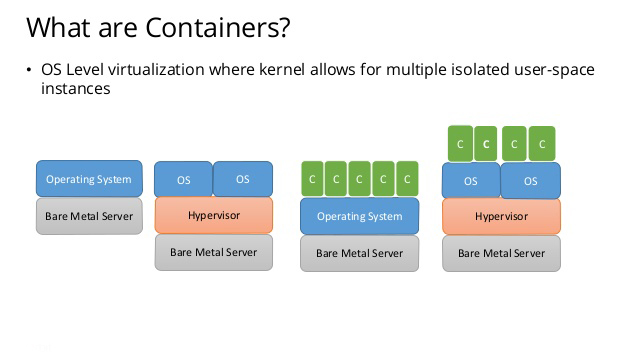
\includegraphics[width=\textwidth]{Figures/que-son-contenedores.jpg}
  \end{center}
  \caption{Un concepto básico de que son los contenedores \citep{Teimouri-Davoud-OS-level-virt}.}
  \label{que-son-contenedores}
\end{figure}

\begin{figure}
  \begin{center}
      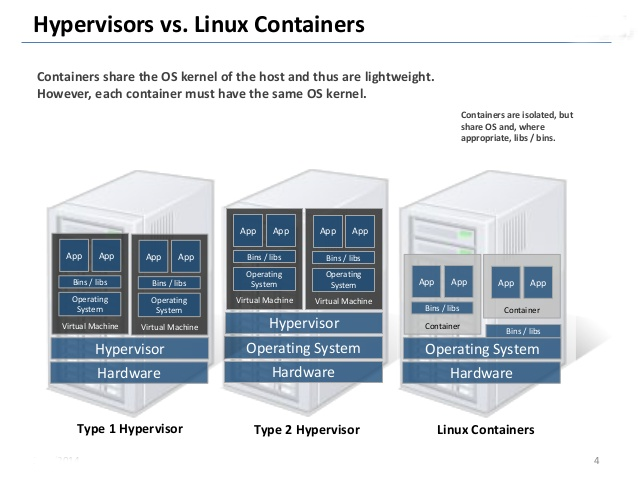
\includegraphics[width=0.75\textwidth]{Figures/differencia-hipervisores-contenedores.png}
  \end{center}
  \caption{La diferencia que abarca contenedores de los tipos de hipervisores \citep{Teimouri-Davoud-OS-level-virt}.}
  \label{differencia-hipervisores-contenedores}
\end{figure}

Debido al hecho de que muchas veces cada máquina virtual necesita su propio hardware virtual y también sistema operativo, se termina consumiendo mucho más RAM y ciclos de CPU de tal manera que un servidor típicamente puede soportar dos a tres veces más servicios si están en contenedores en lugar de si son virtualizados \citep{Teimouri-Davoud-OS-level-virt}. La diferencia se puede ver en la figura \ref{differencia-hipervisores-contenedores}.

\begin{figure}
  \begin{center}
      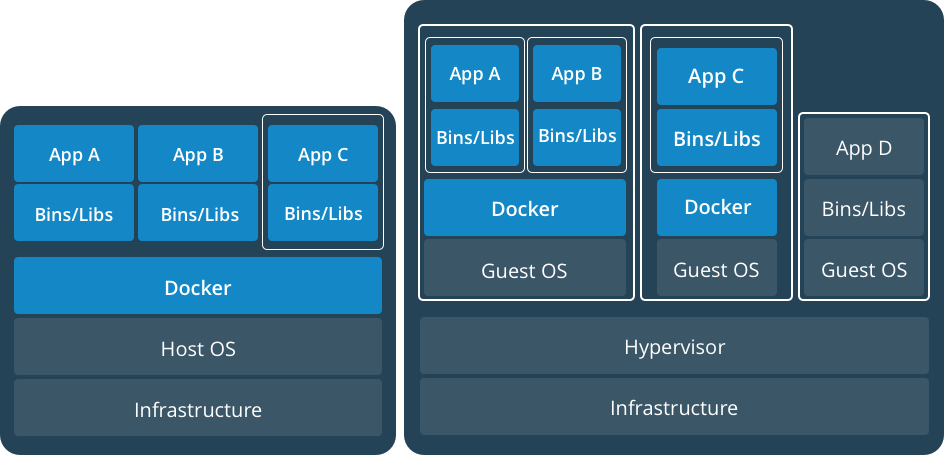
\includegraphics[width=0.75\textwidth]{Figures/contenedores-vms.png}
  \end{center}
  \caption{La diferencia entre contenedores nativas y dentro de una máquina virtual. \citep{Docker-Containers}}
  \label{contenedores-vms}
\end{figure}

Entre las ventajas de contenedores está que permiten tener ambientes aislados livianos para prevenir conflictos de dependencias y estandarizar versiones utilizadas en ambientes de desarrollo y producción mientras que al mismo tiempo requieren mucho menos recursos que una máquina virtual. Las mismas se pueden levantar casi instantáneamente a diferencia de máquinas virtuales que requieren tiempo para arrancarse. Como se puede ver en la figura (contenedores-vms), también se puede tener un motor de contenedores dentro de una máquina virtual, el cual ofrece beneficios como mayor aislamiento (seguridad) y flexibilidad al momento de migrar aplicaciones entre servidores \citep{Docker-Containers}.

La estandarización que ofrece la contenerización ayuda abstraer sistemas operativos que están en los servidores (permitiendo mayor flexibilidad de despliegue),  permite mayor escalabilidad si la aplicación es diseñada para eso, es fácil de versionar dado que los archivos de configuración que describen los contenedores muchas veces son de texto plano y es muy orientado a arquitecturas compuestas por servicios como SOA o las arquitecturas de Microservicios debidos a que estas ya tienen componentes donde es fácil saber dónde poner la frontera de cada contenedor \citep{DigitalOcean-Docker-Ecosystem}.

Para tener seguridad adicional, también se puede ocupar contendores dentro de máquinas virtuales aisladas como se puede observar en la figura \ref{contenedores-vms} \citep{Docker-Containers}.

\subparagraph{Docker}
Docker es una plataforma más popular hoy en dia para contenedores. Se puede usar para eliminar problemas de dependencias entre equipos de desarrolladores, para aumentar la capacidad computacional de equipos y también para desplegar de una forma más ágil, rápida y segura. Con contenedores de Docker, toda la complejidad está dentro del contenedor, facilitando su compilación, la forma en que son compartidos y ejecutados, lo que hace fácil que cualquier persona que tenga los archivos de configuración necesarias puede levantar la aplicación en minutos en lugar de en horas \citep{Docker-What-Is}.

La arquitectura de Docker permite funcionar con cualquier tecnología. La estandarización y facilidad que ofrece permite mejor colaboración entre miembros de un equipo. Por defecto Docker se trata de ser lo más seguro, flexible y extensible posible mientras que al mismo tiempo no necesitar cambios para que un proveedor de software no necesita realizar cambios ni casarse con la tecnología \citep{Docker}.

Frente la percepcion comun de que Docker es insegura, McKendrick y Gallagher ofrecen buenas practicas para el uso de Docker en ambientes de produccion como: 
\begin{itemize}
  \item Utilizar solo contenedores confiables que se puede entender sus contenidos en base a un Dockerfile
  \item Ejecutar el mismo contenedor con y sin un sistema ficheros y despues realizar una comparacion entre los dos para auditar comportamiento.
  \item Auditorias de Contenedores con:
  \begin{itemize}
    \item Docker Bench Security
    \item El uso de servicios de terceros:
    \begin{itemize}
      \item Quay
      \item Clair
    \end{itemize}
  \end{itemize}
  \item Una aplicacion en cada contenedor
  \item Instalaciones minimalistas de lo minimo necesario
  \item Control de quien puede enviar commandos al servicio de Docker
  \item Utilizar la version mas actual de Docker
  \item Utilizar restriciones de recursos
  \item Restringir el nivel de permisos con que se ejecuta el contenedor
  \item Reducir el superficie de ataque dentro del contenedor en no montar archivos criticos del sistema host dentro del contenedor
\end{itemize}
Aunque los autores son muy claros en especificar que Docker no es un sistema de virtualizacion dan estos consejos, listados previamente, entre otros de estos para tener mayor seguridad \citep{McKendrickGallagher201707}.

% TODO: Tecnologias de gestion de virtualizacion
% TODO: OpenStack
% TODO: Kubernetes

\subsubsection{Protocolo de Túnel}
Un túnel es una técnica de permitir acceso remoto a recursos en una red a los cuales normalmente no se tendría acceso desde afuera. Se puede realizar esto en la capa 2 de redes con los protocolos como L2TP, PPTP y L2F quienes buscan encapsular paquetes previo a su viaje entre redes y desencapsularlos en ambos lados del túnel. Puede ser una solución económica para todos los involucrados ya que permite montar varios VPNs en la misma infraestructura física \citep{Cisco-Tunneling}. Los protocolos de túnel saben transmitir dos tipos de mensajes, aquellos paquetes que encapsulan datos y otros paquetes auxiliares que definen las reglas de reenvío \citep{Kaspersky-Tunneling}. Por esta razón y también la tendencia de estos protocolos de proteger los datos que transmiten con encriptación resulta en una velocidad de transferencia de datos menor que simple envío directo. Algunos otros protocolos de encapsulación buscan reemplazar TCP y UDP en la capa 4 pero su funcionalidad de transportar paquetes entre redes, que de ninguna otra forma serían conectados, es igual y forma un tipo de VPN. Los protocolos SSH y IPSec también tienen esas funcionalidades. Así se puede lograr reenviar puertos para utilizar servicios internos como portales internos de una institución o convertir una máquina con Linux/UNIX en un servidor gráfico para “terminales tontos” \citep{ENP-Tunneling} como los días clásicas de la infancia de UNIX \citep{GeerlingJeff-History-Remote-Access}. Aunque su poder y seguridad lo ha hecho un herramienta común entre profesionales que trabajan con redes \citep{ENP-Tunneling}, también por su misma naturaleza se puede ocultar tráfico y por lo tanto ahora es común que malware y actores maliciosos utilizan esos mismos protocolos para esconder su actividad y realizar actos malvados con un menor riesgo de ser detectados en tiempo real. Por lo tanto, para usuarios normales, se recomienda limitar el uso de estos protocolos \citep{Kaspersky-Tunneling}.

\subsubsection{Criptografía}
Criptografía es una ciencia de proteger datos comunicados que han sido utilizado por miles de años para comunicarse de tal forma que el emisor y receptor pueden enviar y recibir mensajes pero personas intermedias no pueden entender los mensajes en tránsito. Tiene aplicaciones militares, financieros y también en el ámbito tecnológico, sobre todo para el internet, entre otras aplicaciones para los cuales ha sido usado a lo largo de la historia. Cifrar es el acto de ocultar datos y decifrar es la acción opuesta para devolverlos a su estado original \citep{Khanacademy-What-is-Cryptography}.

\paragraph{Criptografía Asimétrica}
Con la introducción de redes y la necesidad de encriptar comunicaciones entre personas quienes nunca se ha habían reunido para llegar a un acuerdo de que usar de llave criptográfica para comunicaciones, se necesitaba una manera de llegar a este acuerdo sin que ningún agente intermedio también sepa la llave criptográfica resultante del acuerdo y por lo tanto se introdujo la necesidad de la criptografía asimétrica \citep{Khanacademy-RSA-1}. Para cumplir con este requisito, el receptor genera una llave privada y llave pública, los cuales son operaciones inversas y publica su llave pública para todos que deseen comunicarse con el mismo. Ahora quienes quieren comunicar con el dueño de la par de llaves ocupan su llave pública para cifrar el mensaje y lo envían. Solo con la llave privada se puede descifrar el mensaje y así como el dueño es el único que tiene esta llave, sólo él puede leer los mensajes enviados \citep{Khanacademy-RSA-1}.

\subsubsection{SSH}
En la infancia de la computación, solo habían computadores centralizados en instituciones grandes. Aún no existía el Internet ni las  redes, estaban en su infancia. Poco a poco se introdujo la idea del terminal tonto y con ello el acceso por varios usuarios a estas mismas computadoras centralizados sobre un LAN institucional. De aquí proviene el concepto de control remoto y en aquella época de redes bien controlados y cableados, no hubo mucho riesgos de seguridad entonces por lo tanto el protocolo de esos tiempos fue Telnet, donde todos los datos, incluyendo usuarios y contraseñas son enviados en texto plano. Con el tiempo se volvió más económico y ubicó la tecnología de tal forma que, junto al Internet, se estaba empezando a usar Telnet en redes de desconocidos y generando situaciones potencialmente maduros para ataques clásicos de análisis o incluso modificación de paquetes en tránsito. Fue frente esta realidad que un Finlandés diseñó e implementó el protocolo SSH \citep{GeerlingJeff-History-Remote-Access}. OpenSSH es una implementación abierta y libre \citep{OpenBSD-OpenSSH-Features} del protocolo SSH, que como se define el protocolo, cifrar su tráfico para proteger contra espionaje, robo de conexión y otros ataques que afectan otros protocolos de una naturaleza similar. El proyecto OpenSSH, para ofrecer la mayor funcionalidad posible tiene integrado funcionalidades de túneles seguros, varios métodos de autenticación, y opciones avanzadas de configuración. Adicional a esto ofrece una variedad de herramientas para la gestión de sus funcionalidades con clientes como los comandos ssh, scp y sftp, gestión de llaves con comandos como ssh-add, ssh-keysign, ssh-keyscan, y ssh-keygen, en adición a servicios en segundo plano como sshd, sftp-server y ssh-agent \citep{OpenSSH}. Hoy en día se puede utilizar SSH para cifrar conexiones en redes que de ninguna otra forma serían cifradas, reenviar tráfico de un servidor gráfico X11 (para tener varios terminales gráficos en una sola máquina servidor \citep{ENP-Tunneling}), reenvío de puertos sobre un canal seguro, fuerte mecanismos de autenticación como claves de único uso y llaves de criptografía asimétrica, reenvío de agentes de autenticación, interoperabilidad con otras versiones y implementaciones del protocolo SSH, y la opción de activar compresión y descompresión de datos en tiempo real para optimizar el consumo de recursos en red \citep{OpenBSD-OpenSSH-Features} \citep{OpenBSD-manpages-SSH}.

\paragraph{Túnel de SSH}
SSH es un protocolo de túnel muy popular \citep{Kaspersky-Tunneling} ya que ofrece mucha flexibilidad para las mismas \citep{OpenSSH} y alta seguridad desde la autenticación para iniciar la conexión y para los datos transferidos en dentro de la conexión \citep{OpenBSD-OpenSSH-Features}. Su facilidad de uso permite con rapidez levantar mini VPNs de un puerto para acceder a puertos de otros equipos los cuales normalmente no serían disponibles, por ejemplo acceder servicios que solo son disponibles en un intranet \citep{ENP-Tunneling}.

\subsubsection{SSL}
SSL es un estándar tecnológico para cifrar tráfico \citep{info.SSL.com-SSL} \citep{GlobalSign-SSL} de protocolos que normalmente no son cifrados por ejemplo HTTP, SMTP e IMAP. Esto se hace con un fin de proteger datos sensitivos transferidos (en adición a asegurar su integridad \citep{info.SSL.com-SSL}) entre un cliente y servidor, los cuales normalmente se transfieren en texto plano y podrían ser leídos por cualquier agente intermedio. El proceso de comunicación se puede encontrar en la figura \ref{SSL-Proceso}. Para iniciarse la conexión cifrada, primero el cliente pide que el servidor se identifica (1) con la llave pública que forma parte de su certificado (2). Una vez que lo tiene, el cliente procede a validar el certificado para ver si confía en su origen (a través de firmas digitales por autoridades centrales) y en caso de que haya confianza, se procede a generar una llave criptográfica para la sesión, lo cual se lo transmite cifrada al servidor con la llave pública del mismo (3). El servidor descifra la clave de sesión con su llave privada de su certificado, avisa el cliente que la transacción ha sido exitosa (4) y ambos proceden a transferir los datos adecuados, cifrados con la llave de sesión que tanto cliente como servidor comparten (5) \citep{DigiCert-SSL}.

\begin{figure}
  \begin{center}
      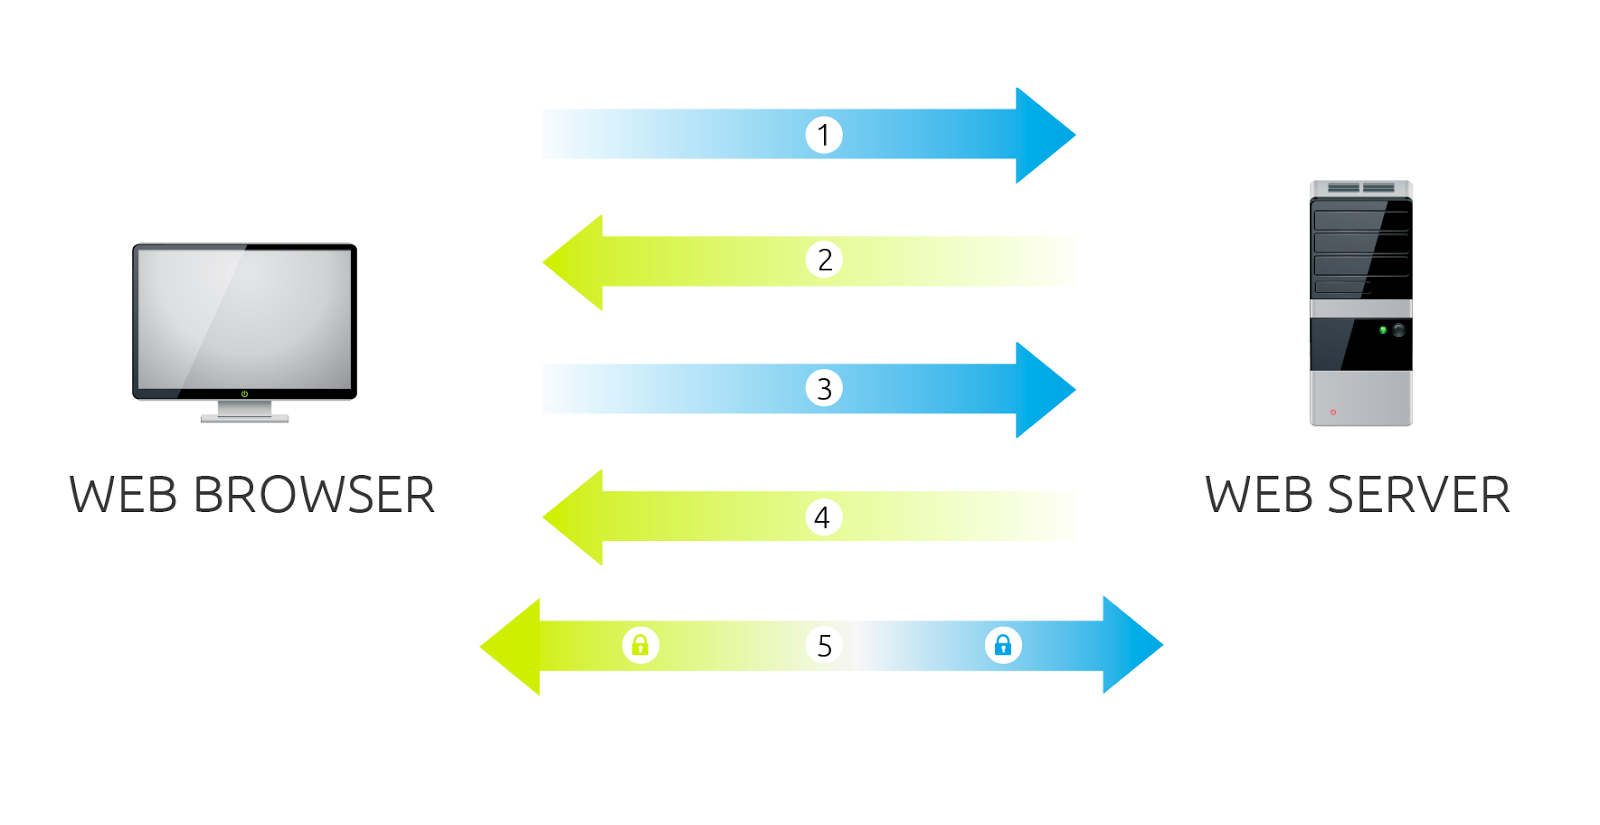
\includegraphics[width=\textwidth]{Figures/ssl-proceso.png}
  \end{center}
  \caption{El proceso para comunicación con el protocolo SSL. \citep{DigiCert-SSL}}
  \label{SSL-Proceso}
\end{figure}

Para ayudar con el proceso de validación, el certificado SSL sabe contener detalles como la llave pública del servidor, el nombre de dominio, nombre de empresa, dirección, ciudad, estado o provincia y país. Es firmado por un autoridad de certificados para dar confianza a los clientes que revisarán el certificado \citep{info.SSL.com-SSL}. Antes de firmar un certificado, una autoridad de certificados primero valida la identidad del servidor que ha realizado la petición para el certificado para que más adelante puede confirmar a clientes que es el mismo servidor \citep{GlobalSign-SSL}.

\paragraph{TLS}
Cuando llegó la versión 4.0 de SSL, se cambió de nombre a TLS versión 1.0 \citep{DigiCert-SSL} para señalar un fuerte cambio de seguridad en cómo se manejan los casos de uso que pueden causar fallos de seguridad en antiguas versiones de SSL como POODLE, DROWN y BEAST que dejan la seguridad que promete SSL inútil y peligroso (ya que las mismas prometen seguridad falsa) \citep{LuxSci-SSL-vs-TLS} \citep{GlobalSign-SSL-vs-TLS}.

\subsection{Tecnologías de la Web}

\begin{table}[h!]
    \begin{tabular}{|p{0.15\textwidth}|p{0.8\textwidth}|}
    	\hline
        Concepto & Definición \\
    	\hline
        URI & Una URI identifica de forma única un recurso que existe en una red como el Internet \citep{Webopedia-URI}. Como se define en el RFC 3986, debe consistir de forma genérica en un:
        \newline
[protocolo de acceso][usuario][clave][dominio][ruta de recurso][parámetros de acceso al recurso]
		\newline
Donde usuario, clave son opcionales y la ruta del recurso y sus parámetros también pueden ser opcionales o innecesarios en casos de protocolos que no requieren el mismo \citep{RFC3986}. \\
        \hline
    	HTTP & HTTP es el protocolo con el cual se intercambia información como peticiones y datos con páginas web en el World Wide Web. Usa un esquema de códigos de error para comunicar tipos de sucesos que pueden ocurrir con el uso del protocolo \citep{ComputerHope-HTTP}. Dentro del protocolo HTTP, se usa verbos que son comandos que dicen que tipo de operación quiere hacer un cliente con relación a un servidor web. HTTP es conocido como un protocolo sin estados ya que dentro del protocolo se desconoce acciones anteriores que se ha tomado en la interacción cliente/servidor \citep{Webopedia-HTTP}. Algunas tecnologías adicionales de la web se muestran en la tabla (tecnologias-web). \\
        \hline
        HTTPS & HTTPS utiliza el estándar SSL y ahora TLS para cifrar conexiones HTTP entre un cliente y servidor \citep{ComputerHope-HTTP}. \\
        \hline
        API REST & Un API REST es un estilo arquitectónico donde se construye encima del protocolo HTTP para orientar el mismo protocolo a manejar estados. Este mismo estilo arquitectónico se orienta a escalabilidad y sistemas de software grandes \citep{Webopedia-REST}. \\
        \hline
        HTML & HTML es el lenguaje de autoría para páginas en la web. Usa una combinación de cientos de etiquetas predefinidas para definir estructura, formato y posición de contenido \citep{Webopedia-HTML}. \\
        \hline
        CSS & CSS es un lenguaje que permite definir estilos de cómo se presentará HTML. Se dice que son hojas de estilo en cascada porque se puede aplicar varios de ellos “en cascada” a una página de HTML \citep{Webopedia-CSS}. \\
        \hline
        JavaScript & JavaScript es un lenguaje de programación que tiene un fin de permitir que páginas de HTML sean dinámicas y pueden interactuar con el usuario en tiempo real \citep{Webopedia-JavaScript}.. \\
        \hline
    \end{tabular}
	\caption{Algunos de las tecnologías de la web.}
    \label{tecnologias-web}
\end{table}

El cuadro \ref{tecnologias-web} presenta conceptos de varias tecnologías que existen en la web hoy en dia.

\pagebreak

\section{Trabajos Relacionados}
Dentro de la temática de este trabajo de titulación es importante entender trabajos relacionados los mismos que son analizados para en base a ellos entender investigaciones que ya se han realizado y de esta forma aprender de ellos. A continuación se mencionan los siguientes:

\subsection{GitEduERP}
En un trabajo reciente del autor con sus colegas, Marcelo Bravo y Priscilla Vargas, en la Universidad Técnica Particular de Loja, y frente el problema de necesitar ofrecer una ambiente de programación a estudiantes en línea, se realizó un editor de código en línea con sistema de permisos y la capacidad de compartir entre usuarios en un backend de Django y utilizando una librería ACE liberado por Cloud9 IDE que guardaba código editado en una instancia de GitLab CE. Además ofrece chat en línea con una liberia TogetherJS. El resultado era un prototipo que guardaba snippets en GitLab y permite compartir código de una manera muy primitiva entre usuarios. Se llevó el codigo editado en un sistema de control de versiones interna, usando MongoDB. Entre los problemas que se dieron era una falta de tiempo para el proyecto y una alta nivel de complejidad para el mismo lo cual no permitía que se lo termina según su alcance propuesta \citep{UTPL-GitEduERP}.

\subsection{Sistema de Encuestas Online}
En la Universidad Técnica Particular de Loja, para mejorar temas de business analytics, dos autores, Diana Ortega y Juan Carlos Sánchez, se trataron de diseñar procesos de negocio para realizar colección de datos en tiempo real a través de encuestas y analizar las mismas con un fin de ayudar la toma de decisiones estratégicas de negocio en tiempo real. Plantearon soluciones con un fin de optimizar tiempos y recursos a través del uso de soluciones tecnológicas \citep{UTPL-Thesis-Encuestas-Online}. Aunque no se trató de enseñar ni de programar en línea se considera importante este trabajo relacionado debido al hecho de que llevaron a cabo temas de business analytics y uno de las finalidades de este trabajo de titulación.

\subsection{Metodología de Enseñanza con la Web 2.0}
En la Universidad Técnica Particular de Loja, Mauricio Castillo buscó utilizar la manera en que la moda de lectura-escritura en la Web 2.0 se podría crear cursos interactivos con estudiantes online como base de una nueva metodología de enseñanza. Destaca esos temas desde el punto de vista de ingeniería en sistemas para proporcionar soluciones netamente técnicas y estratégicas para dar el mejor aporte posible a quienes deseen implementar un sistema de este tipo. Estos conocimientos fueron aplicados en una materia ''Diseño de Paginas Web dinamicas con PHP'' en la modalidad abierta y a distancia de la misma universidad para comprobar la validez de la metodología desarrollado lo cual se encontró que al aplicar la metodología de integrar tecnologías de la web 2.0 y aumentar la interacción estudiantil dentro del curso, se pudo aumentar un grado significativo el porcentaje de estudiantes que aprobaron la materia \citep{UTPL-Thesis-Edu-Web-2}.

\subsection{Xen Web-based Terminal for Learning}
Los autores, Abdullah Almurayh y Sudhanshu Semwal de IAENG, propusieron e implementaron una arquitectura de cliente-servidor para la distribución de recursos educativos y en el proceso enseñar a estudiantes de Linux, programación orientada a la nube y gestión de nubes/servidores. Su aplicación web ofrece terminales SSH donde cada estudiante y docente disponía de una máquina virtual de tal forma que tenían su propio ambiente con permisos de superusuario y al mismo tiempo eran aislados de la infraestructura real y de los demás usuarios, motivo por el cual se podía dar una solución flexible y a su vez segura.

Como hipervisor ocuparon un sistema de Xen que controlan remotamente con su servidor de aplicación (servidor web). El enfoque del trabajo era garantizar seguridad mientras que al mismo tiempo dar ambientes con permisos completos donde estudiantes pueden experimentar y aprender sin restricciones mientras al mismo tiempo ser aislados y prevenir el mal uso o de alguna forma maliciosa.

La parte de seguridad se implementó con un validacion de comandos y eliminación de caracteres especiales que se podrían usar para escapar las restricciones establecidas previamente. De esta forma se logró realizar un sistema útil para administradores, docentes y estudiantes dentro del ámbito educativo. El sistema solo se implemento un comando, xe, para gestión del hipervisor Xen atrás y los autores dejaron como trabajo futuro mejorar la seguridad a futuro debido a que no lo vean como algo completo la seguridad actual \citep{almurayh2014xen}.

\section{Sistemas Similares}
De la misma manera que se analiza la parte de trabajos relacionados, es importante conocer también el contexto actual del mercado para ver las alternativas que ofrece la competencia y saber si ya hay alguna solución que sea de mayor beneficio a la universidad que el mismo sistema que se plantea (y por tal razón sería más factible implementar dicha solución en lugar de desarrollar algo nuevo). Se presenta a continuación las iniciativas investigadas:

\subsection{Repl.it}
Repl.it es una plataforma en línea, desarrollado por Neoreason Inc., para escribir y probar código en tiempo real como un IDE en línea. Su producto tiene un componente educativo que permite integración con otros sistemas de aprendizaje, organización por aulas, texto que guía las tareas, calificación automática de tareas a través de pruebas unitarias entre otras características que mejoran la interacción entre docentes y sus alumnos en su aprendizaje de código. Actualmente usa “máquinas completas de linux” para soportar “más de 30 lenguajes” de una manera “fiable y segura”. Como sistema completa ofrece muchas de las funcionalidades que se esperan de un sistema de este tipo como integración LTI,  ejecucion de codigo en linea, soporte para muchos lenguajes, calificación basado en pruebas unitarias entre otros. Pero tanta funcionalidad viene con un precio alto que reduce la accesibilidad al mismo para las instituciones educativos \citep{Repl.it-Home}.

\subsection{io.livecode.ch}
Io.livecode.ch, desarrollado por Nada Amin, es un plataforma prototipo que convierte repositorios públicos de GitHub en tutoriales interactivos y documentados de programación. Permite la ejecución de código en contenedores de Docker en tiempo real. El mismo utiliza máquinas virtuales alojados en DigitalOcean y permite la extensión por terceras personas con más tutoriales  \citep{io.livecode.ch}. El problema del mismo es que no lleva estados, como ambiente de programación en línea estática, solo lleva los datos del momento sin persistirlos y por lo tanto no ofrece factibilidad dentro del alcance del proyecto actual. El mismo hecho de que lleva Docker como su tecnología de virtualización, según Amin, también baja la seguridad de la aplicación y genera graves vectores de ataque dentro del mismo.

\subsection{Cloud9 IDE}
Cloud9 IDE, desarrollado por una empresa incorporado con el mismo nombre, ofrece un espacio de trabajo personal rápido y escalable (pero administrado por la misma empresa) basado en contenedores de Ubuntu encima de Docker para cada usuario, con soporte para 40 lenguajes de programación. Permite ver aplicaciones web en tiempo real con una variedad de navegadores y sistemas operativos. También permiten conectarse a servidores privados del usuario por SSH para utilizar estos en lugar de los servidores que ellos proveen. También tiene la capacidad de compartir código entre varios usuarios bajo permisos de lectura o lectura y escritura, permitiendo que los mismos editan en tiempo real (visible a todos) y que pueden comunicarse a través de chat. El mismo código, una vista previa de ello o su versión completa también se puede compartir públicamente con usuarios que no pertenecen a la plataforma. Todo esto es con un fin de reemplazar todo el ambiente de desarrollo local con un entorno completamente en la nube; ofrece un terminal, editores avanzados de código, división de pantalla, un debugger, temas, personalización de atajos, comandos communes, modo vim y modo sublime para el editor y un editor de imágenes. Cloud9 IDE está orientado más a profesionales y por lo tanto aún no ofrece tan buena integración con sistemas educativas \citep{Cloud9-Home}.

\subsection{GitLab}
GitLab, desarrollado por GitLab Inc. con un conjunto de miembros de una comunidad de software abierta, en adición a ser un servidor de Git, y por lo tanto llevar un control de versiones de los datos que aloja, también ofrece otras características asociados con entornos profesionales de desarrollo como seguimiento de incidentes, revisión de código, un IDE para editar código en línea, la capacidad de tener wikis asociado con proyectos, un sistema de integración continua para probar, compilar y desplegar código en una variedad de ambientes. Su versión de pago también soporta el consumo de un servidor de LDAP para autenticar usuarios, hooks de Git para tomar acciones personalizadas en respuesta a eventos de Git y capacidades para auditoria por parte de administradores \citep{GitLab}. Además, GitLab puede importar proyectos de otros plataformas y servidores de Git a través de una URI, gestión de snippets, ramas protegidas, un API que permite controlar al servidor de GitLab y un registro de contenedores de Docker asociados con cada proyecto. Por tener un enfoque sumamente de guardar código no ofrece caracteristicas tan fuertes ni para desarrollar en linea ni para ejecutar en línea aunque si soporta otros plataformas de integración continua \citep{GitLab-Features}.

\subsection{OverLeaf}
Overleaf es una plataforma en línea, desarrollado por Writelatex Limited en Londres del Reino Unido, para editar y publicar de forma colaborativo documentos de \LaTeX{}. Permite editar \LaTeX{} directamente o usar un editor WYSIWG para quienes no conozcan bien el sistema \TeX{}. La plataforma compila el documento de \LaTeX{} en tiempo real como se lo va editando para disponer una vista previa con los últimos cambios y de la misma forma avisa de errores que genera al compilador. Como es una plataforma en línea, se puede editar el mismo documento varias personas al mismo tiempo desde distintos clases de dispositivos y cómo el sistema que respalda los documentos es un motor completo de \LaTeX{}/\TeX{}, permite una gran variedad de tipos de documentos y contenido en ellos \citep{Overleaf}. También se integra Overleaf con Git ya que el mismo dispone de un servidor interno de Git para interactuar con sus proyectos a través de este sistema de control de versiones \citep{Overleaf-Git}. Obviamente aunque es un plataforma muy potente para lo que hace también es completamente especializado para el fin de realizar documentos de \LaTeX{}.

\subsection{Google Drive}
Google Drive como servicio de la misma empresa Google ofrece 15 Gigabytes de Almacenamiento gratis para guardar cualquier tipo de archivo, los mismos que pueden ser compartidos con cualquier persona para facilitar colaboración entre personas. Tiene para editar en línea documentos, hojas de cálculo, presentaciones, formularios (para hacer encuestas), dibujos y más con una API que permite mayor expansión por terceros. También controla las versiones de forma automática para que se puede volver a revisar versiones anteriores y quienes han introducido cambios y como fueron los mismos cambios. Además en caso de requerir acceder ciertos archivos sin internet, se puede señalar a la plataforma de Google Drive que se deben sincronizar en segundo plano cada vez que hay internet para también tener la disponible y actualizada cada vez que se encuentre sin conexión. Está orientado completamente al desarrollo de documentos como paquete de ofimática y por lo tanto ofrece poca utilidad para escribir codigo \citep{Google-Drive-Usage}.

\pagebreak
\section{Discusion}
A continuación, se recapitula los trabajos relacionados y sistemas similares previo al fase de análisis y diseño de una solución en el próximo capítulo.

\subsection{Comparación de Trabajos Relacionados}

En el cuadro \ref{trabajos-relacionados-comparacion} se ve las diferencias entre los trabajos relacionados y los campos del trabajo actual en donde se aplica cada uno de ellos. Tanto GitEduERP como Xen Web-based Terminal for Learning Virtualization permiten a estudiantes editar y persistir código en línea a diferencia del Sistema de Encuestas Online que solo era para recolectar y analizar datos y la metodología de enseñanza online con la web 2.0 que no implementa ninguna parte de enseñar la parte práctica de programación en línea. Para enseñar a estudiantes en línea solo dos trabajos relacionados se tratan de eso; Metodología de Enseñanza con la Web 2.0 que buscaba aplicar tecnologías como los blogs para aumentar la participación estudiantil dentro de las materias a distancia y con ello aumentar su aprendizaje medido a través de la métrica de sus notas en una materia de programación y Xen Web-based Terminal for Learning Virtualization que a diferencia de los demás trabajos relacionados ocupó máquinas virtuales (de Xen) para dar ambientes completos y no tan restringidos a estudiantes para permitir su aprendizaje libre en línea con aspectos de virtualización, programacion y Linux.

\begin{table}[h!]
	\small
    \begin{tabular}{|p{0.17\textwidth}|p{0.105\textwidth}|p{0.105\textwidth}|p{0.15\textwidth}|p{0.15\textwidth}|p{0.17\textwidth}|}
        \hline
            & Editar Código en Línea & Persistir Código en Línea & \mbox{Recolección} y \mbox{Análisis} de \mbox{Datos} para \mbox{decisiones} \mbox{estratégicas} en tiempo real & Metodología de \mbox{Enseñanza} Online & Ambientes Virtualizados \\
        \hline
        GitEduERP & x & x & & & \\
        \hline
        Sistema de Encuestas Online & & & x & & \\
        \hline
        Metodología de \mbox{Enseñanza} con la Web 2.0 & & & & x & \\
        \hline
        Xen Web-based Terminal for Learning \mbox{Virtualization} & x & x &  & x & x \\
        \hline
    \end{tabular}
	\caption{Comparación de Trabajos Relacionados.}
    \label{trabajos-relacionados-comparacion}
\end{table}

\subsection{Comparación de Sistemas Similares}
\begin{table}[h!]
	\small
    \begin{tabular}{|p{0.16\textwidth}|p{0.115\textwidth}|p{0.105\textwidth}|p{0.15\textwidth}|p{0.15\textwidth}|p{0.17\textwidth}|}
        \hline
            & Escribir Código Online & Probar Código Online & Integración LTI & Sistema de Autocalificación & Compilación en Tiempo Real \\
        \hline
        Repl.it & Si & Si & Si & Si & No \\
        \hline
        io.livecode.ch & Si & Si & No & No & No, pero si permite ejeccución de código en linea \\
        \hline
        Cloud9 IDE & Si & Si & No & No & Si para ciertos lenguajes \\
        \hline
        GitLab & Si & No & No & No & No \\
        \hline
        Overleaf & Solo \LaTeX & Solo \LaTeX & No & No & Si, \LaTeX \\
        \hline
        Google Drive & No, \mbox{solo} se lo \mbox{considera} \mbox{como} texto & No & No & No & No \\
        \hline
    \end{tabular}
	\caption{Comparación de Características Generales entre \mbox{Sistemas} Similares.}
    \label{comparacion-sistemas-similares-1}
\end{table}

En el cuadro \ref{comparacion-sistemas-similares-1} se ve las características básicas que se considera para un sistema de este tipo. Dentro de esta comparacion, se ve que Repl.it es la mejor alternativa debida a que soporta todas las características menos la compilación en tiempo real (que podría venir a ser una desventaja que empeora el rendimiento del sistema.

\begin{table}[h!]
	\small
    \begin{tabular}{|p{0.16\textwidth}|p{0.105\textwidth}|p{0.16\textwidth}|p{0.15\textwidth}|p{0.15\textwidth}|p{0.13\textwidth}|}
        \hline
            & Control \mbox{Interno} de \mbox{Versiones} & Integración de algún \mbox{sistema} de \mbox{control} de versiones & Sistema de \mbox{Permisos} & Sistema de \mbox{Compartir} & Compartir / Editar en Tiempo Real \\
        \hline
        Repl.it & No & No & Si, basado en docente / alumno & No & No \\
        \hline
        io.livecode.ch & No & No & No & Todo es Público & No \\
        \hline
        Cloud9 IDE & Si & No & Si, \mbox{basado} en \mbox{usuarios} & Si, \mbox{basado} en \mbox{usuarios} & Si \\
        \hline
        GitLab & Si & Si, Git & Si, \mbox{basado} en \mbox{usuarios} y grupos & Si, \mbox{basado} en \mbox{usuarios} y grupos & No \\
        \hline
        Overleaf & Si & Si, Git & Si, \mbox{basado} en \mbox{usuarios} & Si, \mbox{basado} en \mbox{usuarios} & Si \\
        \hline
        Google Drive & Si & No & Si, \mbox{basado} en \mbox{usuarios} & Si, \mbox{basado} en \mbox{usuarios} & Si \\
        \hline
    \end{tabular}
	\caption{Comparación de Características Sociales entre Sistemas Similares.}
    \label{comparacion-sistemas-similares-2}
\end{table}

En el cuadro \ref{comparacion-sistemas-similares-2} se ve vuelta aspectos sociales de cada sistema, entre ellos cómo funcionan las dinámicas de compartir código y interactuar entre usuarios. Aqui Repl.it sale perdiendo con muy pobre suporte para compartir entre varios usuarios. Los sistemas que son mejores en estos aspectos, por ejemplo GitLab, Overleaf y Google Drive no son tan optimizados a escribir código en línea o a ejecutar el mismo.

\begin{table}[h!]
	\small
    \begin{tabular}{|p{0.15\textwidth}|p{0.15\textwidth}|p{0.15\textwidth}|p{0.15\textwidth}|p{0.15\textwidth}|p{0.15\textwidth}|}
        \hline
            & Control Completo sobre \mbox{ambiente} de ejecución de código & Acceso \mbox{Remoto} al ambiente de Ejecución de Código & Sistema de Documentación & API sobre HTTP(S) & Acceso fuera de línea \\
        \hline
        Repl.it & Si para \mbox{instalación} de \mbox{dependencias} & No & Si, \mbox{documentación} del ejercicio & Si, \mbox{pero} \mbox{está} \mbox{cerrado} a nuevos clientes & No \\
        \hline
        io.livecode.ch & Si, script de Bash & No en \mbox{tiempo} real & Si, HTML & No \mbox{mantiene} estados & No \\
        \hline
        Cloud9 IDE & Si, Terminal & Si, SSH & No, fuera de \mbox{documentos} en el servidor & Si & No \\
        \hline
        GitLab & No & No & Si, Wikis con GitHub Markdown & Si & Si, si es que se ha bajado todo anteriormente con Git \\
        \hline
        Overleaf & No & No & No, todo el sistema es de \mbox{documentación} & Si & Si, si es que se ha bajado todo anteriormente con Git \\
        \hline
        Google Drive & No & No & No, todo el sistema es de \mbox{documentación} & Si & Si \\
        \hline
    \end{tabular}
	\caption{Comparación de Características Avanzadas entre \mbox{Sistemas} Similares.}
    \label{comparacion-sistemas-similares-3}
\end{table}

En el cuadro \ref{comparacion-sistemas-similares-3}, se compara las diferencias entre los aspectos más avanzados de cada uno de los sistemas similares. Aquí no hay ni ganadores ni perdedores. Repl.it ofrece una solucion robusta pero que falta alguna forma de acceso fuera de línea. io.livecode.ch ofrece un sistema basico de documentacion y ejecución basado en HTML, pero no maneja estados y no ofrece interactividad en tiempo real.

Adicionalmente, Cloud9 sufre de las mismas problemas de faltar usabilidad sin conexión y de no disponer de una solución robusta de documentación. GitLab y Overleaf ofrecen acceso a través de Git de sus contenidos, abriendo la posibilidad de trabajar sin conexión, pero Overleaf no es para código exactamente. GitLab ofrece el mejor solucion de documentación a través de sus Wikis, pero esos no se visualizan al mismo tiempo que el código. Y Google Drive ofrece la mejor solución para trabajar sin conexion, pero el plataforma es para documentos, no para código.

Al final, ninguna de los sistemas similares alcanza el nivel de funcionalidad que se requiere y por lo tanto, aunque se puede estudiar los mismos para ver que hacen bien y que hacen mal, es necesario, a partir del próximo capítulo, analizar y diseñar e implementar una solución nueva que satisface las necesidades institucionales que hay actualmente.
